\section*{Methods}


%\section{ Barcode Deconvolution Using a Graph-Based Model}
\label{sec:barcode-deconvolution}

We have developed a graph based algorithm to subdivide reads from the same Read Cloud into groups that, ideally, solve the barcode deconvolution problem. %We term these groups {\bf Enhanced Read Clouds}.

The core intuition behind our approach is that reads from the same Read Cloud from the same fragment will tend to overlap with similar sets of reads from other Read Clouds. Critically, if the total genome length in a sample is large enough, a pair of Read Clouds is unlikely to contain reads from more one overlapping genomic region. In what follows, we justify this statement.


%Though each set of reads with the same barcode can contain reads from several fragments (5-20), it is unlikely that two sets of reads with two different barcodes would contain reads from multiple separate overlapping fragments. If multiple reads with the same barcode overlapped with reads that had another barcode it would suggest that the original reads came from the same fragment.

\subsection*{Mathematical Justification of the Model}
\label{sec:math-model}
We have developed a simple model to justify our statement that reads from the same fragment will overlap with reads from similar sets of Read Clouds. This model is similar to empirical results and can be used to inform the parameters used for deconvolution.

First, we develop a model for drawing fragments of DNA from genomes in a metagenomic sample. For simplicity, We model each microbial genome $G_i$ in a metagenome $G$ as a discrete collection of exactly $N_g$ fragments $\vec{F_i}$ where $i$ is an index numbering each genome in the metagenome. $N_g$ is the same for all genomes. The probability of selecting a given fragment $F_{i,j}$ (where individual fragments are indexed by $j$) from a given microbial genome $G_i$ is given by a uniform distribution. We model the probability of selecting a given genome as a Geometric distribution; this choice is motivated by observations of real microbial communities that tend to be dominated by 1-2 species with a long tail of lower abundance species. 

\[\]

The probability of selecting a particular fragment $F_{i,j}$ given that we are drawing fragments from genome $G_i$ is % In our model this probability is constant for all genomes.

\[ P(F=F_{i,j} | G_i) = \frac{1}{N_g } \forall i \in 1:|G| \]

For simplicity we assume the abundance of genomes $G_1, G_2, \cdots$ is sorted in descending order by their index. The probability of selecting a given genome $G_i$ is

\[ P(G = G_i) = \frac{1}{ 2^i } \]

This gives us the probability of drawing a single given fragment $F_{i,j}$ without a given genome.

\[ P(F_{i,j}) = \frac{1}{N_g \times 2^i} \]

The probability that two fragments $F_{w,x}, F_{y,z}$ are the same given that their genomes $G_w, G_y$ are the same is

\[ P( F_{w,x} = F_{y,z} | G_w = G_y) = \frac{1}{N_g} \]

The probability that two genomes $G_w, G_y$ are the same is given below. In real communities this is an approximation that improves as the total number of species increases.

\[ P(G_w = G_y) = \lim_{|G| \rightarrow \infty} \sum_{i=1}^{|G|} \frac{1}{2^{2i}} = \frac{1}{2}\]

Let $p_f$ be the probability that two fragments $F_{w,x}, F_{y,z}$ are the same without conditioning on a given genome. We have

\[ p_f = P( F_{w,x} = F_{y,z}) = \frac{1}{2N_g }  \]

Second, we develop a generative model for assembling a Read Cloud from a set of fragments. We model each Read Cloud as a selection of $N_f$ fragments drawn from the set of all possible fragments. We refer to the set of fragments in a given Read Cloud as $R_i$ For simplicity we do handle the case where two Read Clouds both contain multiple fragments from the same class, this case is very unlikely with parameters relevant to our scenario (1 in 25,000 with the parameters given below). 

\[\]

Let $X(k)$ be the probability that two Read Clouds $R_i$ and $R_j$, both with $N_f$ fragments, share exactly $k$ fragments. In other words any fragment in $R_i$ overlaps with at least one fragment in $R_j$ and vice versa. 


We have 

\[  X(0) = P(|R_i \cap R_j| = 0) = (1 - p_f)^{N_f^2} \]

This is simply because none of the $N_f^2$ possible pairs of fragments (i.e. one in $R_i$ and one in $R_j$) overlap.

We also have


\[  X(1) = P(|R_i \cap R_j| = 1) = 2N_f(1 - (1-p_f)^{N_f})(1-p_f)^{N_f(N_f-1)} - N_f^2p_f(1-p_f)^{N_f^2 - 1} \]

Here exactly one fragment in $R_i$ overlaps with one or more fragments in $R_j$ or vice versa. While it is extremely unlikely that we observe overlap of a fragment in $R_i$ with more than one fragment in $R_j$, we handle this case in our equations because this is allowed in our approximate generative model. We have $2N_f$ possibilities to select a fragment in either $R_i$ or $R_j$. This fragment must overlap with at least one fragment in the other Read Cloud (i.e. the term $1 - (1-p_f)^{N_f}$). No other pair of fragments must overlap (i.e. the term $(1-p_f)^{N_f \cdot (N_f-1)}$) and because we double-counted cases where exactly one fragment in $R_i$ overlaps with exactly one in $R_j$ we subtracted the term $ N_f^2p_f(1-p_f)^{N_f^2 - 1}$.

%\[  X(k) = P(|B_i \cap B_j| = k) = \binom{N_b}{k}^2 \cdot k! * p_f^k * (1 - p_f)^{N_b^2 - k} \]

The probability that two Read Clouds share more than one fragment is

\[  X(\geq 2) = P(|R_i \cap R_j| > 1) = 1 - X(0) - X(1) \]

We choose reasonable, conservative (compared to our observed data), values for all parameters $N_f = 5, N_g = 100, |G| = 10$ and obtain the following estimates.

\[ p_f = \frac{1}{200} \]
\[ X(0) \approx 0.8822, X(1) \approx 0.113,  X(\geq 2) \approx 0.0048 \]
\[ \frac{X(1)}{X(\geq 2)} > 23\]

We find that it is about 23 times more likely to have exactly one overlapping fragment between two Read Clouds than multiple overlapping fragments in our mathematical model. We verified this through simulation and obtained a similar ratio of 1 to 40 (the discrepancy occurs because of how our simulation samples the geometric distribution). This is true even with conservative parameters chosen to minimize the ratio. This is important because it means we are likely to avoid a large number of spurious connections between genomic regions that could lead to poor deconvolution. However, this model does not account for the fact that individual fragments may have similar sequences, which is a major source of noise for Minerva. To reduce this noise, we use the parameters of this model to justify removing any overlaps that occur far more often than expected.

On average, each fragment in a dataset is only fractionally covered at a rate of $C_r$ (with a read depth of 1). While the precise coverage might vary between fragments this parameter can be used to estimate the size of overlaps between fragments and their expected sparsity. Two long fragments would be expected to overlap at $C_r^2$ points in their overlap. In cases where fragments overlap much more frequently than $C_r^2$ over their lengths it can be inferred that the sequence present is too repetitive or common to be useful for deconvolution. 

These facts are used in Minerva to filter connections between repetitive regions, restrict overlaps to regions of a certain length, and to heuristically filter comparisons between Read Clouds unlikely to have significant overlap. This carries practical performance benefits and reduces errors.

\subsection*{A Graph Based Algorithm for Barcode Deconvolution}
\label{sec:graph-model}

\begin{figure}
  \begin{center}
    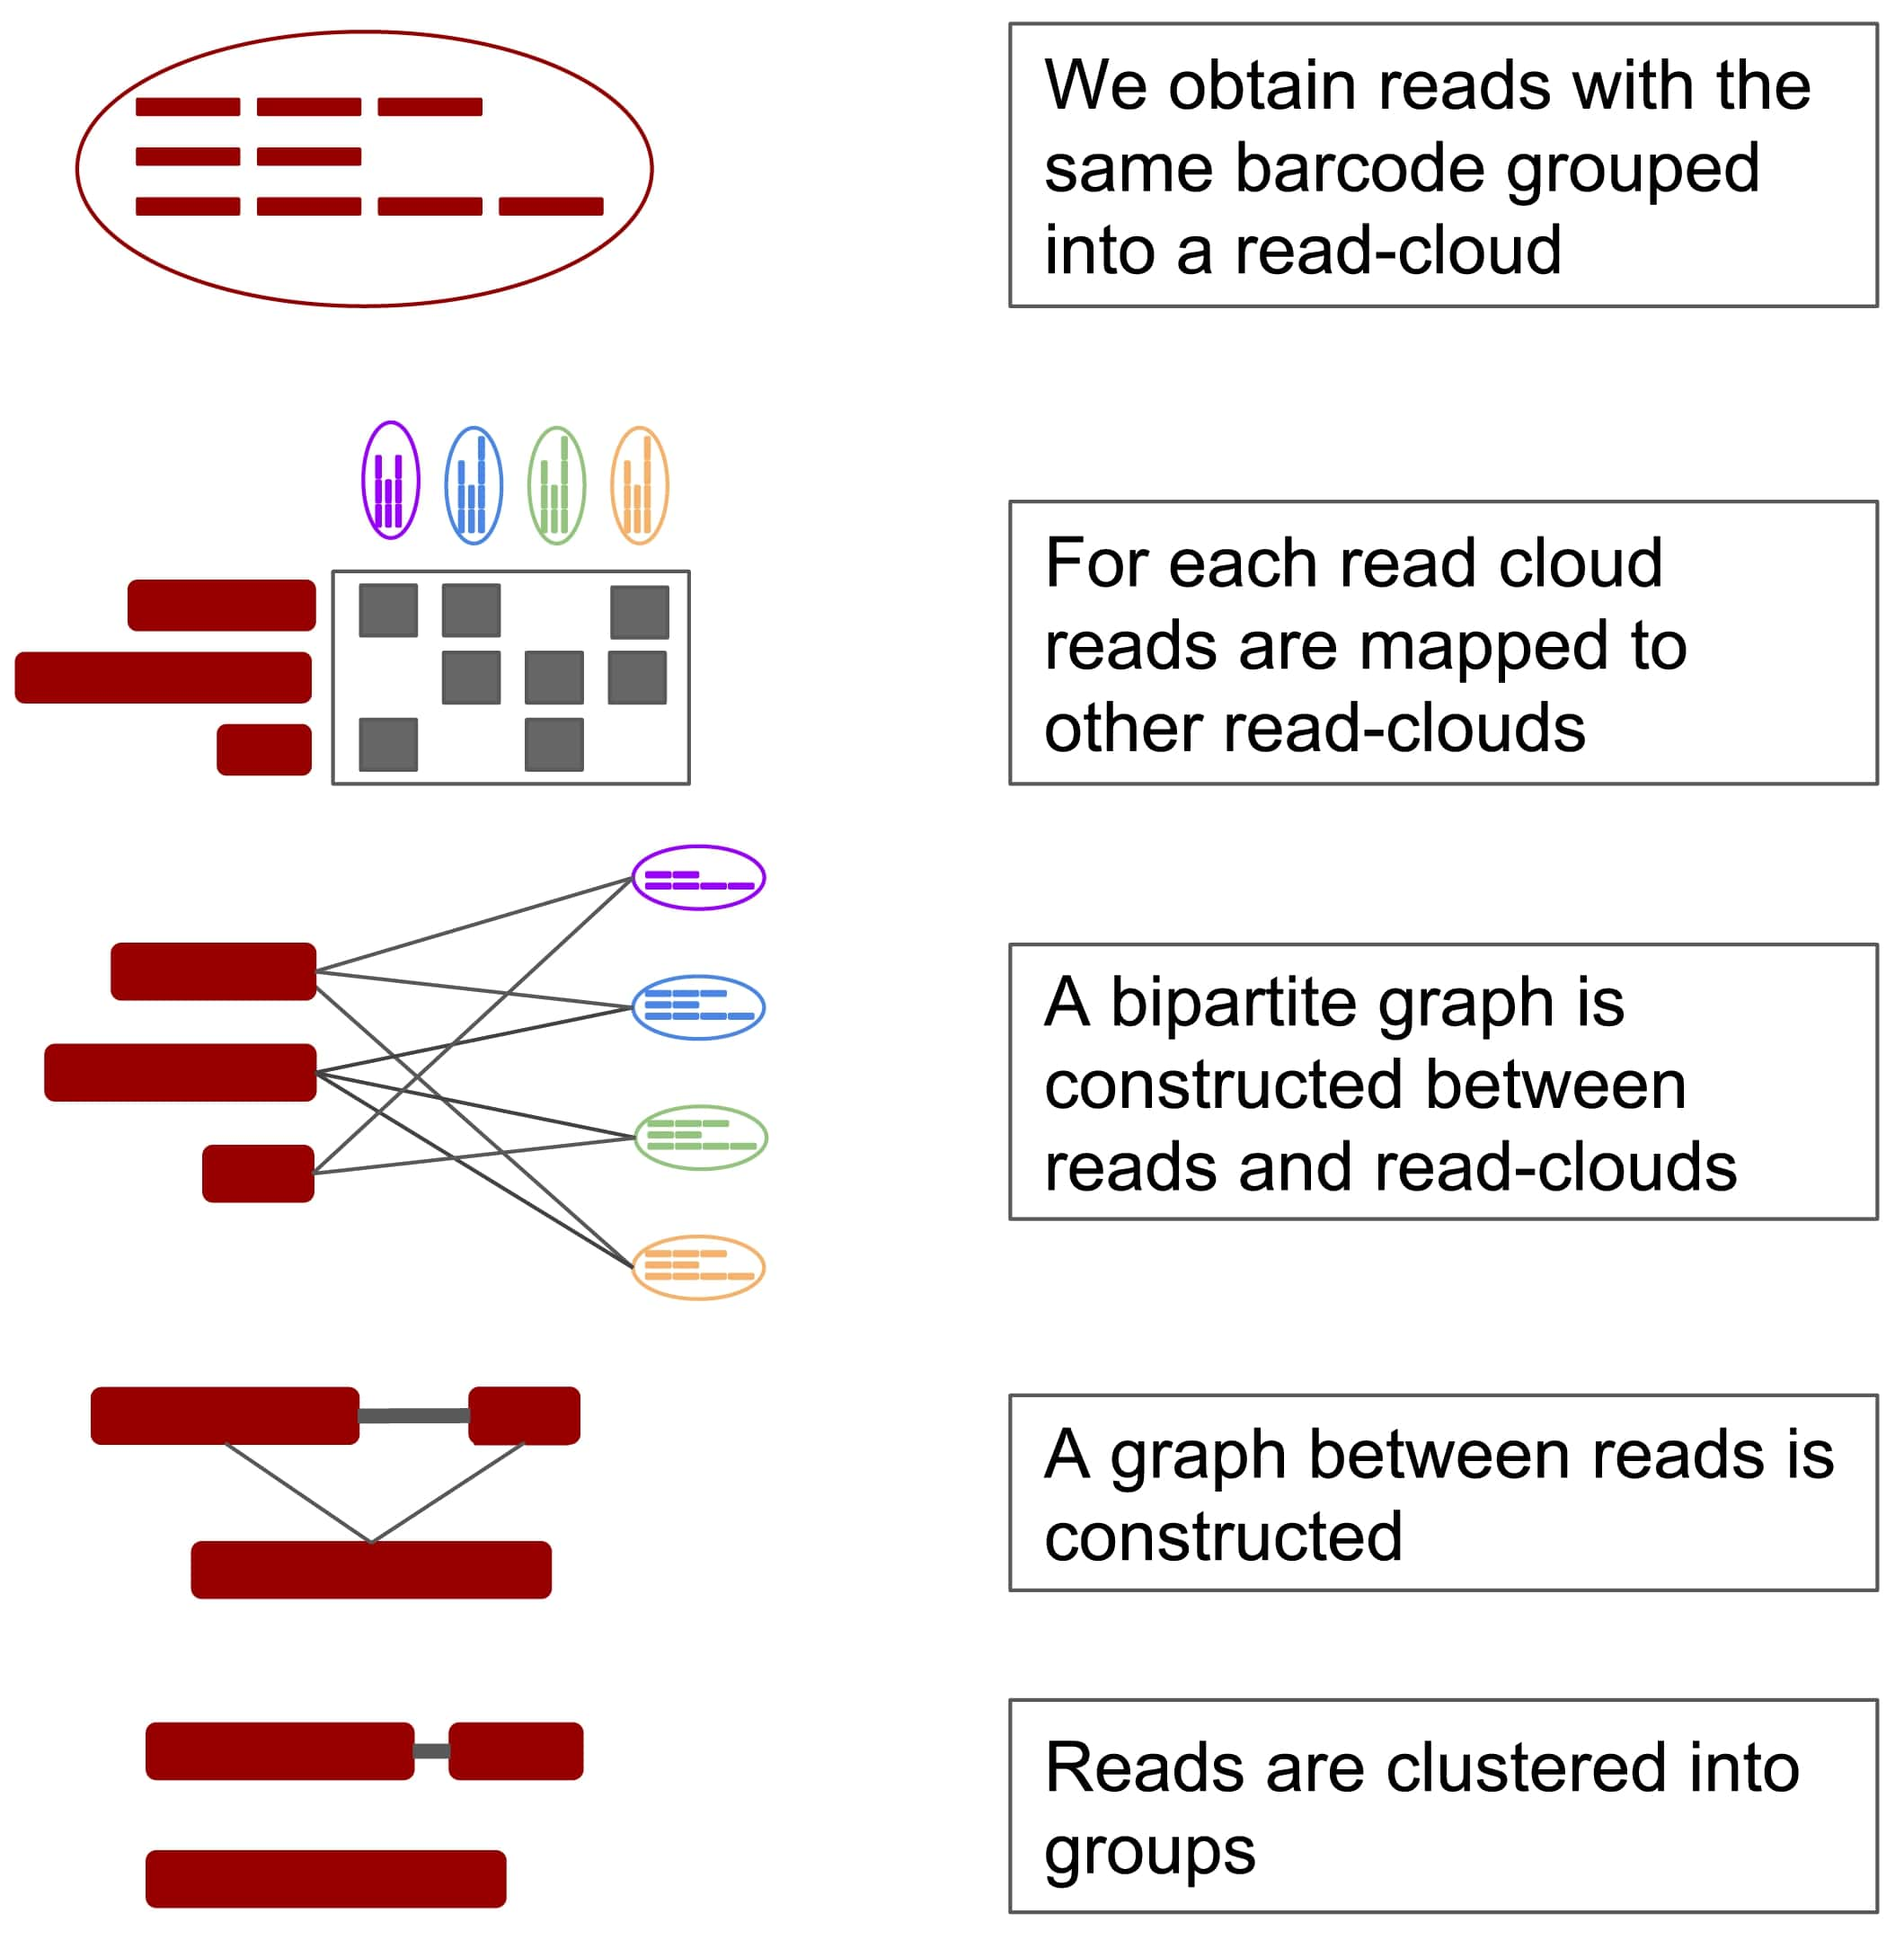
\includegraphics[width=0.8\textwidth]{figures/algorithm_figure.jpg}
%	\vspace{-20pt}
	\caption{\small{Processing steps for a single read cloud. From top 1) Fragments are sequenced and tagged with 3' barcodes 2) Reads in a given read cloud are mapped to reads in other read clouds using minimizing \textit{k}-mers 3) A bipartite graph between reads and other read clouds is constructed 4) A graph between reads that map to the same read clouds is constructed 5) Reads are clustered into groups  }}
    \label{fig:pipe}
  \end{center}
%  \vspace{-20pt}
 % \vspace{1pt}
\end{figure}

\subsubsection*{Summary}
\label{algo}

We have developed a graph based algorithm that effectively deconvolves the reads within a given Read Clouds. The model constructs a bipartite graph between all reads with a given Read Cloud and all other Read Clouds. Reads have an edge to a Read Cloud if they are found to contain a \textit{k}-mer that is specific to exactly one read in the foreign Read Cloud. Once the bipartite graph is constructed Read Clouds and reads with too many or too few edges (by user supplied parameters) are removed. The filtered bipartite graph is used to construct an adjacency matrix between reads and the matrix is clustered into groups of reads. This algorithm is $O(n^2)$ over the number of Read Clouds, though we note that the number of Read Clouds is a constant for each specific technology that could be used. 

The specific steps in our algorithm are as follows:

\begin{enumerate}
\item Read Clouds are parsed, Read Clouds below a certain size (dropout) are dropped. Each read in each Read Cloud is parsed into a set of minimum sparse \textit{k}-mers
\item Each Read Cloud above a certain size (anchor dropout) is compared to all other read clouds. The read cloud being compared is called the 'anchor'
\item A bipartite graph is constructed between the reads in the anchor and all other read clouds based on \textit{k}-mer overlap
\item The bipartite graph is reduced to a graph between reads in the anchor
\item The read graph is broken into discrete clusters which are output as solutions to the barcode deconvolution problem
\end{enumerate}

\subsubsection*{The Model}

Initially each Read Cloud in a given dataset is parsed into a set of minimizing \textit{k}-mers (figure \ref{fig:pipe} part 1). Global counts for \textit{k}-mers are retained. Once parsing is complete, \textit{k}-mers that occur exactly once or many times more than the average (10 times more, by default) are discarded. Singleton \textit{k}-mers cannot occur in more than one barcode and \textit{k}-mers that are too common tend to create false positives (these \textit{k}-mers appear to originate from low complexity or conserved regions). This process is analogous to removing stop words in Natural Language Processing applications. A map of \textit{k}-mers to reads is retained for each Read Cloud.

After parsing, the set of reads in a given Read Cloud is compared to every other Read Cloud (figure \ref{fig:pipe} part 2). Comparisons between Read Clouds that share too many \textit{k}-mers are discarded as these likely represent low complexity or evolutionarily conserved regions as opposed to real overlaps. Comparisons between Read Clouds that share too few \textit{k}-mers are also rejected to improve performance. The intersection of the \textit{k}-mer sets between the given Read Clouds and all Read Clouds that passed filtering is calculated.

A bipartite graph is constructed by creating nodes for every read in the Read Cloud being processed and every Read Cloud that was not filtered out (figure \ref{fig:pipe} part 3). Edges are only added between read-nodes (left nodes) and Read Cloud-nodes (right nodes). An edge is drawn between a read-node and a Read Cloud-node if, and only if, the read shares a \textit{k}-mer with the given Read Cloud. This is a fast proxy measure for read overlap. Finally, any Read Cloud-node with degree above a given threshold is discarded.

Each bipartite graph representing the reads from a given Read Cloud is given a final round of filtering where reads that matched too many foreign Read Clouds are removed based on a user supplied threshold. The filtered bipartite graph is converted to an adjacency matrix of reads where the similarity between reads is equivalent to the number of Read Clouds that both reads overlapped with (figure \ref{fig:pipe} part 4). This adjacency matrix is converted to a binary matrix by setting all values below a user supplied threshold to zero and all remaining values to one (figure \ref{fig:pipe} part 5). 

All connected components in the binary matrix are found. Connected components consisting of single reads are discarded, the remaining components define clusters. This process is analogous to DBSCAN~\citep{Ester1996} for graphs.



\subsection*{Information Theory Bounds on Barcode Deconvolution}

We note that the barcode deconvolution problem on the graph based model we describe in section \ref{sec:graph-model} is analogous to the community recovery problem \citep{Girvan2002} in Information Theory. In particular, 3' barcodes provide linkage information between pairs of reads. We use this linkage information to construct a graph between the reads being deconvolved with the expectation that reads from the same fragment will have a better chance of being linked than reads from different fragments. Formally we say that two reads are connected with probability $p$ if they are from the same fragment and probability $q$ if they are from different fragments. Termed differently $p$ is the true positive rate while $q$ is the false positive rate.

For clarity we note that this model is distinct from the model we developed previously to justify why overlaps between read clouds were likely to be useful for deconvolution.

If we make a simplifying assumption that all fragments in our Read Cloud produce equal numbers of reads we can use the formula determined by ~\citep{Hajek2016} to determine the minimum connectivity of linking 3' barcodes necessary to deconvolve our reads. We define the number of reads per fragment as $\frac{N_r}{N_f}$, where $N_r$ is the total number of reads in a Read Cloud and $N_f$ is the number of fragments in the given Read Cloud.

For the community recovery problem ~\citep{Hajek2016} have provided a lower bound on the size of graph that can be accurately clustered given values of $p$ and $q$, regardless of the algorithm used. If a graph is smaller than this threshold it is unlikely that it will be possible to distinguish clusters from spurious edges. This boundary requires us to assume that all fragments with the same 3' barcode produced equal numbers of reads. Using the definitions above this definition we can apply the following inequality to Read Cloud deconvolution:

\[  \frac{N_r}{\log N_r}( \sqrt{p} - \sqrt{q})^2 > N_f \]

Using the model developed in \ref{sec:math-model} and a simulation we estimate the maximum true positive rate $p$ to be 0.998 and we estimate the minimum false positive rate $q$ to be $\frac{p}{15} = 0.067$. We note that these values do not account for multiple sources of error, notably sequence homology, and should be interpreted as a best case scenario. Using these values we can reduce the previous equation:

\[ 0.549\frac{N_r}{\log N_r} > N_f \]

If a barcode deconvolution graph does not meet this inequality it is  unlikely that it will be possible to accurately reconstruct all clusters. More generally this formula can be used to estimate the minimum number of reads and maximum error rates which can lead to effective barcode deconvolutions. In principle, this inequality should apply to all barocode deconvolution algorithms that can be formulated as a graph. However different algorithms may have different values of $p$ and $q$. We also note that the above formula is based on asymptotic behavior for graphs with thousands of nodes. We observed that typical deconvolution graphs in our model have fewer than 50 nodes. 

\subsection*{ Minimum Sparse Hashing}
\label{sec:MSH}

\begin{figure}%{r}{0.3\textwidth}
%  \vspace{-20pt}
  \begin{center}
   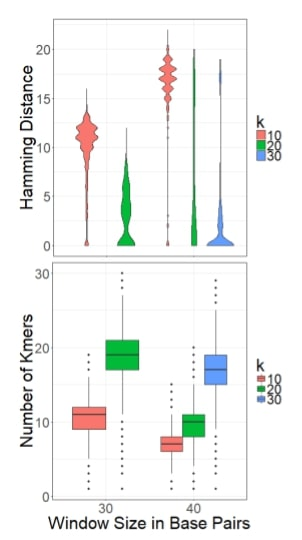
\includegraphics[width=0.4\textwidth]{figures/minsparse_fig.jpg}
%	\vspace{-5pt}
	\caption{\small{Top, Hamming distance between windows that share minimizing \textit{k}-mers, using various parameters. Bottom, number of representative minimizing \textit{k}-mers per read}}
    \label{fig:minsparse_fig}
  \end{center}
 % \vspace{-60pt}
 % \vspace{1pt}
\end{figure}

Minerva frequently tests whether pairs of reads overlap. Many solutions to finding overlaps between reads exist, such as: sequence clustering algorithms, sequence aligners, and \textit{k}-mer matching. These techniques typically make trade offs between overall performance and error rates. Since Minerva is meant to be relatively fast and can tolerate some errors we elected to use a minimal sparse hash of \textit{k}-mers to match read pairs. This technique reduces the number of unique \textit{k}-mers Minerva uses to find overlaps which reduces runtime and RAM usage.

Minimum sparse hashing was originally developed independently for biological sequence search and natural language document search \citep{Marcais2017,Schleimer2003} (in natural language search the technique is referred to as winnowing). While the original application of this technique in biology defined minimization as the lexicographic minimum of a set of sequences we use a uniform random hash function to determine the minimal sequence in a set. This is a common practical enhancement recently detailed by~\citep{Orenstein2016}. 


Minimum sparse hashing for sequences takes three parameters, a length $k$, a window size $w$, and a hash function $h$. Given a set $K$ of $n, n \geq w$ \textit{k}-mers, the min-sparse hash computes the hash $h$ of each \textit{k}-mer then selects the \textit{k}-mer with the smallest numerical hash from each consecutive set of $w$ \textit{k}-mers in $K$. The final set of minimizers is the unique set of \textit{k}-mers generated, $W$. Each consecutive window shares $w-1$ \textit{k}-mers so there is a good chance that each window shares the same minimum with its predecessor. Formally $W = \{\min(h(k) \forall k \in K_{(i,i+w)}) \forall i \in 0:(n-w)\}$. This algorithm guarantees that any pair of reads with an exact overlap of at least $w + k - 1$ bases will share at least one minimum sparse \textit{k}-mer while drastically reducing the number of \textit{k}-mers which must be stored in memory (figure \ref{fig:minsparse_fig}). In certain implementations minimum sparse \textit{k}-mers may also improve performance by allowing a \textit{k}-mer that can be stored in a single 64 bit cell ($ k\leq 32$) of memory to represent a longer sequence.

Minimum sparse \textit{k}-mers are prone to false positives when presented with similar, but not identical, runs of $w$ bases in read pairs. We measured this phenomenon by comparing all \textit{k}-mers of length $w$ from pairs of reads that share a minimum sparse hash. Figure \ref{fig:minsparse_fig} shows the minimum hamming distance for windows of length $w$ between reads that share a minsparse hash. When $k$ is larger the average hamming distance is smaller though outliers persist. Small values of $k$ produce many distant false positives. Raising $k$ from 20 to 30 ($w=40$) improved accuracy and precision to the point where false positives could be controlled using downstream techniques.



The mathematics that underlie minimum sparse hashing may also be used to efficiently approximate the overlap between sets, another important operation for Minerva. We did not use this technique in our current implementation of Minerva but plan to explore this for later versions. %maybe move this to conclusion / future work



%\subsection{Practical Uses}

%We directly tested Minerva's ability to deconvolve barcodes from metagenomic samples (section \ref{sec:purity}). No other barcode deconvolution procedures exist so we could not make a direct comparison to other tools. We also show two practical use cases for barcode deconvolution in metagenomics. In future, we expect our barocde deconvolution technique to be used in several other applications of linked-read sequencing including de Bruijn graph based assemblers as well. %However, at the time of writing no robust assembler for linked read metagenomic data has been developed yet.

